\documentclass[t,usenames,dvipsnames]{beamer}
\usetheme{Copenhagen}
\setbeamertemplate{headline}{} % remove toc from headers
\beamertemplatenavigationsymbolsempty

\usepackage{amsmath, tkz-euclide, tikz, xcolor, pgfplots, array}
\usetkzobj{all}
\pgfplotsset{compat = 1.16}
\usetikzlibrary{arrows.meta, calc, decorations.pathreplacing}
\pgfplotsset{every axis/.append style = {axis lines = middle, axis line style = {<->}}}
\pgfplotsset{every tick label/.append style={font=\tiny}}
\everymath{\displaystyle}

\title{Trig Equations}
\author{}
\date{}

\AtBeginSection[]
{
  \begin{frame}
    \frametitle{Objectives}
    \tableofcontents[currentsection]
  \end{frame}
}

\begin{document}

\begin{frame}
    \maketitle
\end{frame}

\section{Solve trigonometric equations}

\begin{frame}{Trig Equations}
    A \alert{trigonometric equation} is one that contains a trig function with variable, such as $\sin x = \frac{1}{2}$.
\end{frame}

\begin{frame}{Trig Equations}
\begin{center}
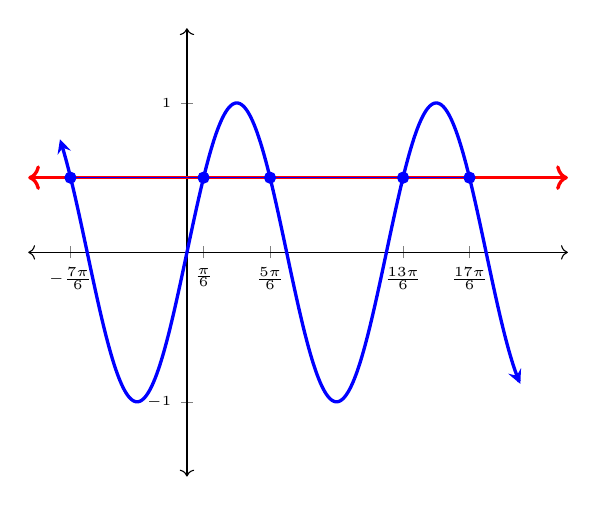
\begin{tikzpicture}
\begin{axis}[
xmin = -5, xmax = 12,
ymin = -1.5, ymax = 1.5,
xtick = {-3.67, 0.524, 2.618, 6.809, 8.901},
xticklabels = {$-\frac{7\pi}{6}$, $\frac{\pi}{6}$, $\frac{5\pi}{6}$, $\frac{13\pi}{6}$, $\frac{17\pi}{6}$}
]
\addplot [<->,>=stealth,very thick,domain=-4:10.5, samples = 300, smooth, blue] {sin(deg(x))}; 
\addplot+ [<->, domain=-5:12, no marks, very thick] {0.5};
\addplot [color=blue, mark=*] coordinates {(-3.67,0.5) (0.524,0.5) (2.618,0.5) (6.809,0.5) (8.901,0.5)};
\end{axis}
\end{tikzpicture}
\end{center}
\end{frame}

\begin{frame}{General Form of Solutions}
The \alert{general form} of this solution is
\[x = \frac{\pi}{6}+2\pi n \quad \text{or} \quad x = \frac{5\pi}{6} + 2\pi n \]   

where $2\pi$ is the \alert{period} of the sine function.  \newline\\  \pause

Since there are an infinite number of solutions, we will usually confine our answers to be between 0 and $2\pi$.
\end{frame}

\begin{frame}{How to Solve a Trig Equation}
    \begin{enumerate}
        \item Get the trig function by itself, if possible.    \newline\\
        \item Solve for the variable using inverse trig.
    \end{enumerate}
\end{frame}

\begin{frame}{Example 1}
Solve each of the following in the interval $[0, 2\pi)$.    \newline\\
(a) \quad $\cos(2x) = -\frac{\sqrt{3}}{2}$
\begin{align*}
    \onslide<2->{2x &= 150^\circ + 360n & 2x &= 210 + 360n} \\[8pt]
    \onslide<3->{x &= 75^\circ + 180n & x &= 105^\circ + 180n} \\[8pt]
    \onslide<4->{x &= 75^\circ, \, 255^\circ & x &= 105^\circ, \, 285^\circ} \\[8pt]
\end{align*}
\onslide<5->{
\[ x = \left\{\frac{5\pi}{12}, \, \frac{7\pi}{12}, \, \frac{17\pi}{12}, \, \frac{19\pi}{12} \right\} \]}
\end{frame}

\begin{frame}{Example 1}
(b) \quad $\csc\left(\frac{1}{3}x-\pi\right) = \sqrt{2}$
\begin{align*}
    \onslide<2->{\frac{1}{3}x - 180^\circ &= 45^\circ + 360n & \frac{1}{3}x - 180^\circ &= 135^\circ + 360n}   \\[8pt]
    \onslide<3->{\frac{1}{3}x &= 225^\circ + 360n & \frac{1}{3}x &= 315^\circ + 360n} \\[8pt]
    \onslide<4->{x &= 675^\circ + 1080n & x &= 945^\circ + 1080n} \\[8pt]
\end{align*}
\begin{center}
    \onslide<5->{No angles between 0 and $2\pi$}
\end{center}
\end{frame}

\begin{frame}{Example 1}
(c) \quad $\cot(3x) = 0$
\begin{align*}
    \onslide<2->{3x &= 90^\circ + 180n & 3x &= 270^\circ + 180n} \\[8pt]
    \onslide<3->{x &= 30^\circ + 60n & x &= 90^\circ + 60n} \\[8pt]
    \onslide<4->{x &= 30^\circ, 90^\circ, 150^\circ, 210^\circ, 270^\circ, 330^\circ & x &= 90^\circ, 150^\circ, \dots} \\
\end{align*}
\[ \onslide<5->{x = \left\{\frac{\pi}{6}, \, \frac{\pi}{2}, \, \frac{5\pi}{6}, \, \frac{7\pi}{6}, \, \frac{3\pi}{2}, \, \frac{11\pi}{6}\right\}} \]
\end{frame}

\begin{frame}{Example 1}
(d) \quad $\sec^2 x = 4$
\begin{align*}
    \onslide<2->{\sqrt{\sec^2 x} &= \pm\sqrt{4} & &} \\[6pt]
    \onslide<3->{\sec x &= 2 & \sec x &= -2} \\[6pt]
    \onslide<4->{x &= 60^\circ, 300^\circ & x &= 120^\circ, 240^\circ} 
\end{align*}

\onslide<5->{\[ x = \left\{ \frac{\pi}{3}, \frac{2\pi}{3}, \frac{4\pi}{3}, \frac{5\pi}{3}\right\} \]}
\end{frame}

\begin{frame}{Example 1}
(e) \quad $\tan\left(\frac{x}{2}\right) = -3$
\begin{align*}
    \onslide<2->{\frac{x}{2} &= \tan^{-1}(-3) + 180n & (\arctan(-3) \approx -143^\circ)}    \\[12pt]
    \onslide<3->{x &= 2\tan^{-1}(-3) + 360n & (2\arctan(-3) \approx -286^\circ)} \\[12pt]
    \onslide<4->{x &= 2\tan^{-1}(-3) + 360^\circ} \\[12pt]
    \onslide<5->{x &= 2\tan^{-1}(-3) + 2\pi  &} 
\end{align*}
\end{frame}

\begin{frame}{Using Algebraic Techniques and Trig Identities}
The following examples make use of trig identities and algebraic techniques to solve the equations.
\end{frame}

\begin{frame}{Example 2}
Solve each in the interval $[0, 2\pi)$  \newline\\
(a) \quad $3\sin^3 x = \sin^2 x$
\begin{align*}
    \onslide<2->{3\sin^3 x - \sin^2 x &= 0 & &} \\[6pt]
    \onslide<3->{\sin^2 x(3\sin x - 1) &= 0 & &} \\[6pt]
    \onslide<4->{\sin^2 x &= 0 & 3\sin x - 1 &= 0} \\[6pt]
    \onslide<5->{\sin x &= 0 & \sin x = \frac{1}{3}} \\[6pt]
    \onslide<6->{x &= 0, 180^\circ & x &\approx 19.471^\circ, 160.529^\circ} 
\end{align*}
\[ \onslide<7->{x = \left\{0, \, \arcsin\left(\frac{1}{3}\right), \, \pi - \arcsin\left(\frac{1}{3}\right), \, \pi \right\}}
\]
\end{frame}

\begin{frame}{Example 2}
(b) \quad $\sec^2 x = \tan x + 3$
\begin{align*}
    \onslide<2->{\tan^2 x + 1 &= \tan x + 3} \\[6pt]
    \onslide<3->{\tan^2 x - \tan x - 2 &= 0} \\[6pt]
    \onslide<4->{(\tan x - 2)(\tan x + 1) &= 0}
\end{align*}
\begin{align*}
    \onslide<5->{\tan x - 2 &= 0 & \tan x + 1 &= 0} \\
    \onslide<6->{\tan x &= 2 & \tan x &= -1}    \\
    \onslide<7->{x &\approx 63.5^\circ, 243.5^\circ & x &= 135^\circ, 315^\circ} 
\end{align*}
\[
\onslide<8->{x = \left\{\arctan(2), \, \frac{3\pi}{4}, \, \pi + \arctan(2), \, \frac{7\pi}{4} \right\}}
\]
\end{frame}

\begin{frame}{Example 2}
(c) \quad $\cos(2x) = 3\cos x - 2$
\begin{align*}
    \onslide<2->{2\cos^2 x - 1 &= 3\cos x - 2} \\
    \onslide<3->{2\cos^2 x - 3\cos x + 1 &= 0} \\
    \onslide<4->{(2\cos x - 1)(\cos x - 1) &= 0}
\end{align*}
\begin{align*}
    \onslide<5->{2\cos x - 1 &= 0 & \cos x - 1 &= 0} \\
    \onslide<6->{\cos x &= \frac{1}{2} & \cos x &= 1} \\[6pt]
    \onslide<7->{x &= 60^\circ, 300^\circ & x &= 0}
\end{align*}

\[
\onslide<8->{x = \left\{ 0, \, \frac{\pi}{3}, \, \frac{5\pi}{3} \right\}}
\]
\end{frame}

\begin{frame}{Example 2}
(d) \quad $\sin(2x) = \sqrt{3}\cos x$
\begin{align*}
    \onslide<2->{2\sin x \cos x &= \sqrt{3}\cos x} \\
    \onslide<3->{2\sin x \cos x - \sqrt{3} \cos x &= 0} \\
    \onslide<4->{\cos x(2\sin x - \sqrt{3}) &= 0} \\
\end{align*}
\begin{align*}
    \onslide<5->{\cos x &= 0 & 2\sin x - \sqrt{3} &= 0} \\
    \onslide<6->{x &= 90^\circ, 270^\circ & 2\sin x &= \sqrt{3}} \\
    \onslide<7->{& & \sin x &= \frac{\sqrt{3}}{2}} \\[6pt]
    \onslide<8->{& & x &= 60^\circ, 120^\circ}
\end{align*}
\end{frame}

\begin{frame}{Example 2}
    \begin{align*}
        x &= 60^\circ, \, 90^\circ, \, 120^\circ, \, 270^\circ \\[12pt]
        \onslide<2->{x &= \left\{\frac{\pi}{3}, \, \frac{\pi}{2}, \, \frac{2\pi}{3}, \, \frac{3\pi}{2} \right\}}
    \end{align*}
\end{frame}

\end{document}
